\documentclass[a4paper,14pt]{article}


%%% Работа с русским языком
\usepackage{cmap}					% поиск в PDF
\usepackage[T2A]{fontenc}			% кодировка
\usepackage[utf8]{inputenc}		% кодировка исходного текста
\usepackage[russian]{babel}	% локализация и переносы
%\usepackage{pscyr}
%\renewcommand{\rmdefault}{ftm}
%%% Дополнительная работа с математикой
\usepackage{amsmath,amsfonts,amssymb,amsthm,mathtools,gensymb,float} % AMS
%% Номера формул
%\mathtoolsset{showonlyrefs=true} % Показывать номера только у тех формул, на которые есть \eqref{} в тексте.
%\usepackage{leqno} % Нумерация формул слева
%\usepackage{rumathgrk1}
%% Перенос знаков в формулах (по Львовскому)
\newcommand*{\hm}[1]{#1\nobreak\discretionary{}
	{\hbox{$\mathsurround=0pt #1$}}{}}
%\usepackage{glonti}
%%% Работа с картинками
\usepackage{graphicx}  % Для вставки рисунков
\graphicspath{{images/}{images2/}}  % папки с картинками
\usepackage{wrapfig} % Обтекание рисунков текстом
\addto\captionsrussian{\def\refname{Список используемой литературы}}
%%% Работа с таблицами
\usepackage{array,tabularx,tabulary} % Дополнительная работа с таблицами
\usepackage{longtable}  % Длинные таблицы
\usepackage{multirow} % Слияние строк в таблице
%%% Теоремы
\theoremstyle{plain} % Это стиль по умолчанию, его можно не переопределять.
\newtheorem{theorem}{Теорема}[section]
\newtheorem{proposition}[theorem]{Утверждение}

\theoremstyle{definition} % "Определение"
\newtheorem{corollary}{Следствие}[theorem]
\newtheorem{problem}{Задача}[section]

\theoremstyle{remark} % "Примечание"
\newtheorem*{nonum}{Решение}
%\pagestyle{empty}
%%% Страница
\usepackage{extsizes} % Возможность сделать 14-й шрифт
\usepackage{geometry} % Простой способ задавать поля
\geometry{top=20mm}
%\geometry{bottom=35mm}
\geometry{left=25mm}
\geometry{right=20mm}
\setlength{\parindent}{1.1cm}

\usepackage{setspace} % Интерлиньяж
\onehalfspacing % Интерлиньяж 1.5
% \doublespacing % Интерлиньяж 2
%\singlespacing % Интерлиньяж 1

\usepackage{lastpage} % Узнать, сколько всего страниц в документе.
\usepackage[usenames]{color}
\usepackage{colortbl}
\renewcommand{\baselinestretch}{1.05}
\usepackage{hyperref}
\usepackage[usenames,dvipsnames,svgnames,table]{xcolor}
\hypersetup{				% Гиперссылки
	unicode=true,           % русские буквы в раздела PDF
	pdftitle={Заголовок},   % Заголовок
	pdfauthor={Автор},      % Автор
	pdfsubject={Тема},      % Тема
	pdfcreator={Создатель}, % Создатель
	pdfproducer={Производитель}, % Производитель
	pdfkeywords={keyword1} {key2} {key3}, % Ключевые слова
	colorlinks=true,       	% false: ссылки в рамках; true: цветные ссылки
	linkcolor=black,          % внутренние ссылки
	citecolor=blue,        % на библиографию
	filecolor=magenta,      % на файлы
	urlcolor=cyan           % на URL
}

\usepackage{bm}
\usepackage{tikz}
\begin{document}
% НАЧАЛО ТИТУЛЬНОГО ЛИСТА
\begin{center}
    {\textsc{Федеральное государственное бюджетное образовательное
            учреждение высшего образования
        }}\\
    {\textsc{Московский государственный университет имени М.В. Ломоносова
    }} \\
    \vspace{0.2cm}
    {\textsc{Механико - математический факультет}}\\
    \vspace{0.2cm}
    {\textsc{Кафедра прикладной механики и управления}}\\
    \hfill \break
    \begin{figure}[h!]
        \centering
        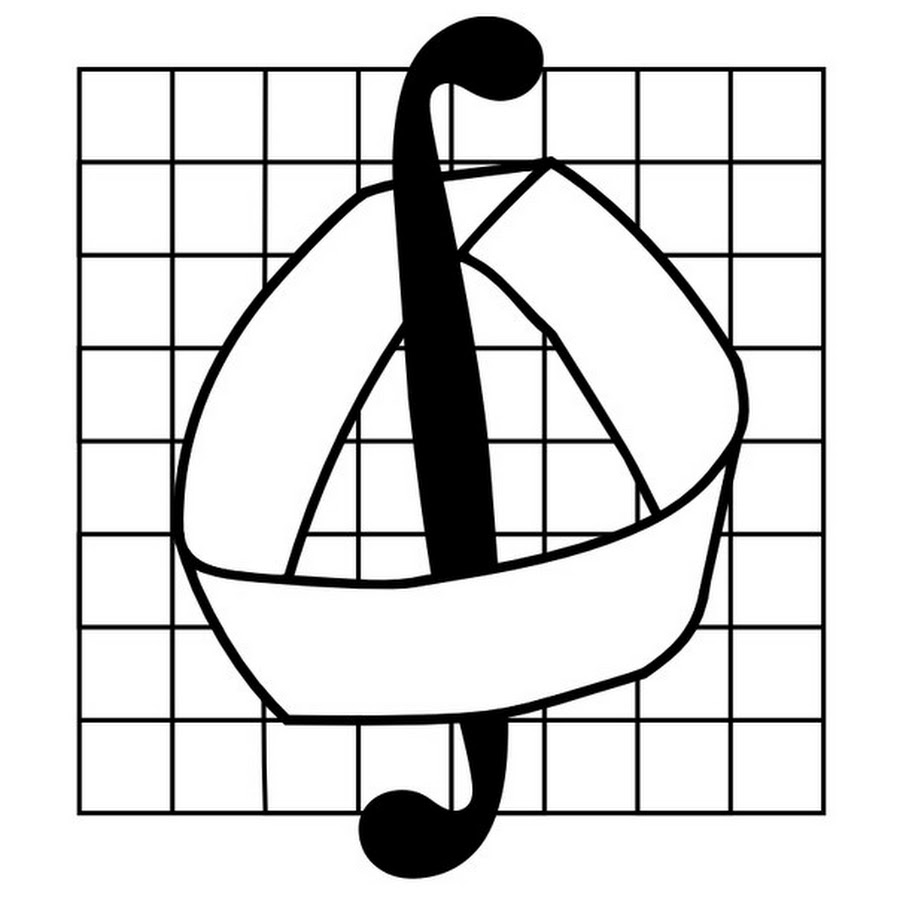
\includegraphics[width=0.30\linewidth]{emblema}
        \label{fig:emblema}
    \end{figure}
    \hfill \break
    \hfill \break
    \large{\textbf{Домашняя работа №2}\\
        \hfill \break Инерциальные навигационные системы
    }
\end{center}

\hfill \break
\hfill \break
\begin{flushright}
    {
        Выполнил: студент группы М -- 1 \\ Романов Андрей Владимирович}
\end{flushright}

\begin{flushright}
    {
        Преподаватель: д.ф.-м.н., \\ Голован Андрей Андреевич}
\end{flushright}
\hfill \break
\hfill \break
\begin{center} {Москва, 2022} \end{center}



\thispagestyle{empty} % выключаем отображение номера для этой страницы
\normalsize{
% КОНЕЦ ТИТУЛЬНОГО ЛИСТА
\newpage
\tableofcontents
\newpage

\section{Задача 1}
\textbf{Задание:}

Введем «замороженный» относительно инерциального пространства трехгранник $M_0x_0^0$,
совпадающий с географическим трехгранником $Mx^0$ БИНС в начальный момент времени $t_0$.
Выведите динамические уравнения движения в абсолютных переменных в осях этого трехгранника.

Предполагается, что в начальный момент времени известны географические координаты $\lambda_0,\varphi_0,h_0$,
скорость относительно Земли ноль, известны начальные значения углов $\psi_0,\vartheta_0,\gamma_0.$

Требуется предъявить все расчетные формулы для определения текущих значений
$\lambda(t),\varphi(t),h(t),V_E(t),V_N(t),V_{UP}(t),\psi(t),\vartheta(t),\gamma(t)$


\textbf{Решение:}
В начальный момент времени трехгранник $M_0x_0^0$
совпадает с географическим трехгранником $Mx^0$, тогда
\begin{equation}\label{koshisystem}
    \left\{ {\begin{aligned}
                 & \lambda(t_0) = \lambda_0 , \hfill \\
                 & \varphi(t_0) = \varphi_0 , \hfill \\
                 & h(t_0)= h_0 . \hfill              \\
            \end{aligned}} \right.
\end{equation}

$A_{x_{0}^{0} \xi}(t)=A_{x_{0} \eta}\left(t_{0}\right) A_{\eta \xi}\left(t_{0}\right)$,

Матрица ориентации $A_{x^0\eta}$ географического трехгранника относительно гринвичского
$$
    A_{x_{0} \eta}\left(t_{0}\right)=\left(\begin{array}{ccc}
            -\sin \lambda_{0}                  & \cos \lambda_{0}                   & 0                \\
            -\cos \lambda_{0} \sin \varphi_{0} & -\sin \lambda_{0} \sin \varphi_{0} & \cos \varphi_{0} \\
            \cos \lambda_{0} \cos \varphi_{0}  & \sin \lambda_{0} \cos \varphi_{0}  & \sin \varphi_{0}
        \end{array}\right),
$$
матрица ориентации гринвичского трехгранника относительно инерциального
$$
    A_{\eta \xi}\left(t_{0}\right)=\left(\begin{array}{ccc}
            \cos u t_{0}  & \sin u t_{0} & 0 \\
            -\sin u t_{0} & \cos u t_{0} & 0 \\
            0             & 0            & 1
        \end{array}\right),
$$
По формуле Эйлера найдем абсолютную скорость:
$$
    v_{x_{0}^{0}}\left(t_{0}\right)=v_{x^{0}}\left(t_{0}\right)=V_{x^{0}}\left(t_{0}\right)-\widehat{u}_{x^{0}}\left(t_{0}\right) x^{0}\left(t_{0}\right)=-\widehat{u}_{x^{0}}\left(t_{0}\right) x^{0}\left(t_{0}\right)
$$
Угловая скорость вращения Земли записанная в $Ox^{0}$ в начальный момент времени:
$u_{x^{0}}\left(t_{0}\right)=\left(\begin{array}{c}0 \\ u \cos \varphi_{0} \\ u \sin \varphi_{0}\end{array}\right)$

Координаты точки $M$ в осях трехгранника $Ox^0$ в начальный момент времени $t_0$:
$x^{0}\left(t_{0}\right)=\left(\begin{array}{c}0 \\ -R_{E 0} e^{2} \cos \varphi_{0} \sin \varphi_{0} \\ R_{E 0}\left(1-e^{2} \sin ^{2} \varphi_{0}\right)+h_{0}\end{array}\right)$

Уравнение Пуассона для матрицы $A_{z^{0} x_{0}^{0}}$ :
$$
    \begin{gathered}
        \dot{A}_{z^{0} x_{0}^{0}}=\widehat{\omega}_{z^{0}} A_{z^{0} x_{0}^{0}}, \quad A_{z^{0} x_{0}^{0}}\left(t_{0}\right)=A^{T}_{x^{0} z^{0}}\left(t_{0}\right) A_{x^{0} x_{0}^{0}}\left(t_{0}\right)=A^{T}_{x^{0} z^{0}}\left(t_{0}\right), \\
        {\footnotesize
        A_{x^{0} z^{0}}\left(t_{0}\right)=\left(\begin{array}{ccc}
                \cos \psi_{0} \cos \gamma_{0}+\sin \psi_{0} \sin \vartheta_{0} \sin \gamma_{0}  & \sin \psi_{0} \cos \vartheta_{0} & \cos \psi_{0} \sin \gamma_{0}-\sin \psi_{0} \sin \vartheta_{0} \cos \gamma_{0}  \\
                -\sin \psi_{0} \cos \gamma_{0}+\cos \psi_{0} \sin \vartheta_{0} \sin \gamma_{0} & \cos \psi_{0} \cos \vartheta_{0} & -\sin \psi_{0} \sin \gamma_{0}-\cos \psi_{0} \sin \vartheta_{0} \cos \gamma_{0} \\
                -\cos \vartheta_{0} \sin \gamma_{0}                                             & \sin \vartheta_{0}               & \cos \vartheta_{0} \cos \gamma_{0}
            \end{array}\right)
        }
    \end{gathered}
$$
Динамические уравнения в осях $M_0x_0^0$
$$
    \left\{\begin{array}{l}
        \dot{x}_{0}^{0}=v_{x_{0}^{0}} \\
        \dot{v}_{x_{0}^{0}}=f_{x_{0}^{0}}+g_{x_{0}^{0}}
    \end{array}\right.
$$
где $f_{x_{0}^{0}}=A_{x_{0}^{0} z^{0}} f_{z^{0}}$ вектор внешней удельной силы, $g_{x_{0}^{0}}=A_{x_{0}^{0} x^{0}} g_{x^{0}}$ - вектор удельной силы тяготения.

Формула Гельмерта, с помощью которой вычисляется значение модуля вектора удельной силы тяжести в географических осях, а также вектор удельной силы тяжести
$$
    g(\varphi)=9.78030\left(1+0.005302 \sin ^{2} \varphi-0.000007 \sin ^{2} 2 \varphi\right)-0.00014-2 \omega_{0}^{2} h
$$
$$
    g_{x^{0}}=\left(\begin{array}{c}
            0                                                   \\
            u^{2}\left(R_{E}+h\right) \sin \varphi \cos \varphi \\
            -g-u^{2}\left(R_{E}+h\right) \cos ^{2} \varphi
        \end{array}\right)
$$
Для интегрирования уравнения Пуассона используем следующий алгоритм:
$$
    \left\{\begin{array}{l}
        \gamma_{z^{0}}=\int_{t_{j}}^{t_{j+1}} \widehat{\omega}_{z^{0}}(\tau) d \tau \\
        A_{z^{0} x_{0}^{0}}\left(t_{j+1}\right)=\left(E+\frac{\sin \gamma}{\gamma} \widehat{\gamma}_{z^{0}}+\frac{1-\cos \gamma}{\gamma^{2}} \widehat{\gamma}_{z^{0}}^{2}\right) A_{z^{0} x_{0}^{0}}\left(t_{j}\right), \quad \gamma=\sqrt{\gamma_{z_{1}^{0}}^{2}+\gamma_{z_{2}^{0}}^{2}+\gamma_{z_{3}^{0}}^{2}}
    \end{array},\right.
$$
У полученной новой матрицы необходимо сохранить ортогонализацию.

Введем интегральную величину $\Delta V_{f}=\int_{t_{j}}^{t_{j+1}} A_{z_{0} x_{0}^{0}}^{T}\left(t_{j+1}\right) f_{z^{0}}(\tau) d \tau$

Получим следующий алгоритм интегрирования
$$
    \left\{\begin{array}{l}
        g_{x_{0}^{0}}\left(t_{j}\right)=A_{x_{0}^{0} \xi} A_{\eta \xi}^{T}\left(t_{j}\right) A_{x^{0} \eta}^{T}\left(t_{j}\right) g_{x^{0}}\left(t_{j}\right) \\
        v_{x_{0}^{0}}\left(t_{j+1}\right)=v_{x_{0}^{0}}\left(t_{j}\right)+g_{x_{0}^{0}}\left(t_{j}\right) \Delta t+\Delta V_{f}                               \\
        x_{0}^{0}\left(t_{j+1}\right)=x_{0}^{0}\left(t_{j}\right)+v_{x_{0}^{0}}\left(t_{j}\right) \Delta t+\frac{1}{2} g_{x_{0}^{0}}\left(t_{j}\right) \Delta t^{2}+\frac{1}{2} \Delta V_{f} \Delta t
    \end{array}\right.
$$
Гринвичские коордианты найдем следующим образом:
$$
    \eta\left(t_{j+1}\right)=A_{\eta x_{0}^{0}}\left(t_{j}\right)\left(O M_{0}+x_{0}^{0}\left(t_{j+1}\right)\right)=A_{\eta \xi}\left(t_{j+1}\right) A_{x_{0}^{0} \xi}^{T}\left(O M_{0}+x_{0}^{0}\left(t_{j+1}\right)\right),
$$
$O M_{0}=x^{0}\left(t_{0}\right)-$ вектор совпадает численно с координатами точки $M$ в системе координат $O x^{0}$ в начальный момент времени.

Долгота находится как $\lambda\left(t_{j+1}\right)=\operatorname{atan} 2\left(\eta_{2}\left(t_{j+1}\right), \eta_{1}\left(t_{j+1}\right)\right)$. Применив меод Ньютона для решения нелинейной системы уравнений найдем $\varphi\left(t_{j+1}\right), h\left(t_{j+1}\right)$
$$
    \left\{\begin{array}{l}
        \sqrt{\eta_{1}^{2}+\eta_{1}^{2}}-\left(R_{E}+h\right) \cos \varphi=0 \\
        \eta_{3}-\left[\left(1-e^{2}\right) R_{E}+h\right]=0
    \end{array}\right.
$$
Теперь можно вычислить $A_{\eta x^{0}}\left(t_{j+1}\right)$ по новым географическим координатам. Географические скорости находятся по формулам:
$$
    \left(\begin{array}{c}
            V_{E}\left(t_{j+1}\right) \\
            V_{N}\left(t_{j+1}\right) \\
            V_{U P}\left(t_{j+1}\right)
        \end{array}\right)=\left(\begin{array}{c}
            v_{E}\left(t_{j+1}\right)-u\left(R_{E}\left(t_{j+1}\right)+h\left(t_{j+1}\right)\right) \cos \varphi\left(t_{j+1}\right) \\
            v_{N}\left(t_{j+1}\right)                                                                                                \\
            v_{U P}\left(t_{j+1}\right)
        \end{array}\right)
$$
$$
    \left(\begin{array}{c}
            v_{E}\left(t_{j+1}\right) \\
            v_{N}\left(t_{j+1}\right) \\
            v_{U P}\left(t_{j+1}\right)
        \end{array}\right)=A_{x^{0} \eta}\left(t_{j+1}\right) A_{\eta \xi}\left(t_{j+1}\right) A_{x_{0}^{0} \xi}^{T} v_{x_{0}^{0}}\left(t_{j+1}\right)
$$


Углы истиннного курса, крена и тангажа находим по формуле $A_{z^{0} \xi}\left(t_{j+1}\right)=A_{z^{0} x_{0}^{0}}\left(t_{j+1}\right) A_{x_{0}^{0} \xi}\left(t_{j+1}\right)$ :
$$
    \begin{aligned}
         & A_{z^{0} \xi}\left(t_{j+1}\right)=\left(a_{i j}\right), \quad \psi\left(t_{j+1}\right)=\operatorname{atan} 2\left(a_{21}, a_{22}\right),                                                                   \\
         & \gamma\left(t_{j+1}\right)=-\operatorname{atan} 2\left(a_{13}, a_{33}\right), \quad \vartheta\left(t_{j+1}\right)=\operatorname{atan} 2\left(a_{23}, \frac{a_{33}}{\cos \gamma\left(t_{j+1}\right)}\right)
    \end{aligned}
$$
\newpage
\section{Задача 2}
\textbf{Задание:}

Пусть баровысотомер доставляет точную информацию о текущей высоте. Выведите
уравнения ошибок демпфируемого вертикального канала. Подберите подходящие
коэффициенты демпфирования.

\textbf{Решение:}

Модельные уравнения демпфируемого вертикального канала
\begin{eqnarray*}
    {\dot  h}'  &=& V_3' - \underline{K_{v_1}\left(h' - h^b\right)}, \nonumber \\
    {\dot V_3}'  &=& (\Omega_2' +  2 u_2') V_1' - (\Omega_1' +
    2u_1') V_2'- g' + f_3' - \underline{K_{v_2}\left(h' - h^b\right) - \Delta {\widetilde f}_3^0} ,\nonumber \\
    \Delta {\dot {\widetilde{f}_3^0 }}  & = & \underline{K_{v_3}\left(h' - h^b\right)}.
\end{eqnarray*}

Пусть доступно измерение баровысотомера
\begin{eqnarray*}
    h^b = h + \Delta h^b ,
\end{eqnarray*}
так как по условию задачи баровысотомер доставляет точные показания, то $h^b=h$

$f_3'$  -- показания "вертикального"\ акселерометра;

$\Delta {\widetilde f}_3^0$ -- оценка нуля "вертикального"\ акселерометра;

$K_{v_1}$, $K_{v_2}$, $K_{v_3}$  --  постоянные коэффициенты алгоритма
демпфирования.
\begin{eqnarray*}
    f_3' =  f_3 + \Delta f_3^0 + \Delta f_3^s,
\end{eqnarray*}
}
где $f_3$ -- истинное значение,
$\Delta f_3^0$ -- постоянное смещение нуля ($(\Delta {\dot f}_3^0 = 0$)  "вертикального" \ акселерометра,
$\Delta f_3^s$ --  шумовая составляющая погрешности измерения.
Идеальные уравнения вертикального канала
\begin{eqnarray*}
    {\dot  h}  &=& V_3, \nonumber \\
    {\dot V_3}  &=& (\Omega_2 +  2 u_2) V_1 - (\Omega_1 +
    2u_1) V_2- g + f_3.
\end{eqnarray*}
Введем

\begin{eqnarray*}
    \Delta h  = h' - h, \qquad \Delta V_3 = V_3' - V_3, \qquad \delta f_3^0 = \Delta f_3^0 - \Delta {\widetilde f}_3^0,
\end{eqnarray*}

где $\delta f_3^0$ имеет смысл ошибки оценивания смещения нуля вертикального акселерометра.

Вычитаем из модельных уравнений идеальные уравнения, в линейном приближении получим (не учитываем вариацию поправки Этвеша)
\begin{eqnarray*}
    \Delta \dot  h  &=& \Delta V_3 - K_{v_1} \Delta h + K_{v_1} \Delta h^b , \nonumber \\
    \Delta \dot V_3  &=&  2 \omega_0^2 \Delta h - K_{v_2} \Delta h + K_{v_2} \Delta h^b + \delta f_3^0 + \Delta f_3^s , \nonumber \\
    \delta {\dot f}_3^0   &=&  K_{v_3} \Delta h - K_{v_3} \Delta h^b
    .
\end{eqnarray*}

Уравнения ошибок примут вид:
\begin{eqnarray*}
    \underbrace{
        \left(
        \begin{array}{c}
            \Delta \dot h \cr
            \Delta \dot V_3 \cr
            \delta {\dot f}_3^0
        \end{array}
        \right)}_{\dot x}
    =
    \underbrace{
        \left(
        \begin{array}{ccc}
            - K_{v_1}             & 1 & 0  \cr
            2\omega_0^2 - K_{v_2} & 0 & 1  \cr
            K_{v_3}               & 0 & 0
        \end{array}
        \right)
    }_{A}
    \underbrace{
        \left(
        \begin{array}{c}
            \Delta h \cr
            \Delta V_3 \cr
            \delta f_3^0
        \end{array}
        \right)
    }_{x}
    +
    \underbrace{
        \left(
        \begin{array}{c}
            \phantom{-} K_{v_1} \Delta h^b \cr
            \phantom{-} K_{v_2} \Delta h^b + \Delta f_3^s \cr
            -K_{v_3} \Delta h^b
        \end{array}
        \right)
    }_{q}
    .
\end{eqnarray*}
Характеристическое уравнение
\begin{eqnarray*}
    \left| \lambda E- A \right| = 0  \Longrightarrow
    \left|
    \begin{array}{ccc}
        \lambda  + K_{v_1}     & -1      & 0 \cr
        -2\omega_0^2 + K_{v_2} & \lambda & -1 \cr
        - K_{v_3}              & 0       & \lambda
    \end{array}
    \right| = 0 .
\end{eqnarray*}
Коэффициенты характеристического уравнения зависят от свободных параметров $K_{v_1}$, $K_{v_2}$, $K_{v_3}$.

Раскроем определитель и получим
$\lambda^3+K_{v_1}\lambda^2+\lambda(-2\omega_0^2 + K_{v_2})-K_{v_3}=0$
Подберем коэффициенты обратной связи таким образом, чтобы характеристическое уравнение имело кратные корни
\begin{eqnarray*}
    \left(\lambda - \lambda_0\right)^3 = 0, \qquad \lambda_0 < 0.
\end{eqnarray*}

$\lambda^3-3\lambda^2\lambda_0+3\lambda\lambda_0^2-\lambda_0^3=0$

Приравняем коэффиценты при соответствующих степенях

$K_{v_1}=-3\lambda_0; -2\omega_0^2 + K_{v_2}=3\lambda_0^2; K_{v_3}=\lambda_0^3$

$K_{v_1}=-3\lambda_0; K_{v_2}=3\lambda_0^2+2\omega_0^2; K_{v_3}=\lambda_0^3$

Для примера возьмем запас устойчивости $\lambda_0=-1$

$\omega_0^2 \simeq 1.543\cdot 10^{-6}$ -- квадрат частоты Шулера.

$K_{v_1}=3; K_{v_2}=3+2\omega_0^2=3.000003; K_{v_3}=-1$

\textbf{Ответ:} $K_{v_1}=3; K_{v_2}=3.000003; K_{v_3}=-1.$
\end{document}